\chapter{Solución}

\section{Arquitectura}

La solución es una librería de Python para generar visualizaciones animadas de estructuras de datos y las operaciones que se realizan sobre estas, que pueda ser usada en un Jupyter Notebook.

La librería le permite al usuario implementar una estructura de datos y agregando la instrumentación provista por la librería le permite generar una visualización animada que muestra las operaciones que se realizaron sobre esa estructura de datos.

Para permitir esto la librería esta compuesta por dos partes: una parte implementada en Python y una parte implementada en JavaScript.

La parte implementada en Python, que correspondería al \textit{back--end}, define la instrumentación para captar las operaciones realizadas sobre la estructura de datos. Se encarga de mantener un registro de todas las operaciones que se realizan sobre la estructura de datos. Este registro se mantiene utilizando una representación de las operaciones primitivas sobre la estructura de datos. Teniendo esto, cuando un usuario quiere generar la visualización este registro de operaciones es serializado y enviado a el \textit{front--end} usando la librería IPython Widgets.

La parte implementada en TypeScript, el \textit{front--end} de la librería, recibe el modelo serializado, deserializa el modelo y genera la visualización a partir de este. Para generar la visualización utiliza la librería D3, que permite manipular el DOM en función de los datos del modelo.

\section{Modelo de datos}

El modelo consiste en una lista de operaciones y metadata de las operaciones registradas. Cada operación está compuesta por una operación primitiva y metadata de la operación. La metadata de la operación consiste en si la operación se debe animar o no y el código fuente que dio origen a esa operación. La operación primitiva puede ser:

\begin{itemize}
    \item{\makebox[3.5cm]{Init(id, value, next)\hfill}}: Inicializar un nodo
    \item{\makebox[3.5cm]{SetValue(id, value)\hfill}}: Asignar el valor de un nodo
    \item{\makebox[3.5cm]{GetValue(id)\hfill}}: Obtener el valor de un nodo
    \item{\makebox[3.5cm]{SetNext(id, next)\hfill}}: Asignar el siguiente de un nodo
    \item{\makebox[3.5cm]{GetNext(id)\hfill}}: Obtener el siguiente de un nodo
\end{itemize}

\section{Front--end}

Como la librería registra las operaciones primitivas no es trivial generar una visualización a partir del modelo, ya que las operaciones registradas no necesariamente representan una operación estándar sobre listas. De hecho estas operaciones definen un grafo dirigido con un grado máximo de 1. Esta representación resulta útil porque permite representar implementaciones incorrectas de una lista enlazada.

Para visualizar por separado las componentes conexas del grafo se deben encontrar los subgrafos conexos a partir de esta representación. En la literatura existen varios algoritmos para resolver este problema, pero por simplicidad se decidió acotar la librería al caso donde el grafo es áciclico, es decir, un bosque. De esta manera, todos los nodos que no tienen ningún arco que apunte a ellos son puntos de entrada. Además, todos estos puntos de entrada definen una lista conexa que no tiene conexiones con otras listas. Entonces, podemos visualizar cada una de estas componentes conexas como una lista.

Para generar la animación se visualiza en orden cada operación primitiva que se obtiene del \textit{front--end} (animándola o no dependiendo de los metadatos de la operación). Para cada operación primitiva primero se obtienen las listas conexas usando el algoritmo descrito previamente, luego se genera una lista donde cada elemento tiene la información asociada a un nodo y finalmente usando D3js se anima la transición desde la versión previa de esta lista hasta la actual.

Los datos asociados a cada nodo son: el índice de la lista a la que pertenece, el largo de la lista a la que pertenece, su índice dentro de la lista a la que pertenece, su identificador único y su valor.

Teniendo la lista, usando D3js se asocian los nodos de la visualización a cada elemento en esta lista usando el identificador del elemento. La animación tiene dos fases: primero se anima la actualización de los nodos existenes y luego se anima la entrada de nuevos nodos.

En la primera fase se transiciona con una animación desde la posición anterior de los nodos a la posición dada por los datos actualizadas asociados a cada nodo y se actualizan los valores que hayan cambiado. En la segunda fase se hace un \textit{fade in} de los nuevos nodos en las posiciones correspondientes. Es importante el orden de estas fases porque si se hace en otro orden los nodos entrantes podrían aparecer detras de nodos preexistentes.

\section{Back--end}

El backend se encarga de proveer la instrumentación necesaria para que el usuario pueda generar visualizaciones de las estructuras de datos que ha implementado. Usando esta instrumentación mantiene un registro de las operaciones primitivas realizadas sobre la estructura de datos y cuando el usuario quiere visualizar el resultado serializa este registro y lo envia al \textit{front--end}.

Para esto la librería provee dos \textit{decoradores} ---azúcar sintáctica de Python para aplicar funciones a las definiciones de clases o funciones--- \textit{node} y \textit{container}. El primero de estos denota la clase que representa el nodo de la lista enlazada, mientras que el segundo denota la clase que contiene una referencia al primer nodo de la lista. En el código~\ref{lst:ejemplo-uso} se puede ver un ejemplo del uso de estos decoradores y en la figura~\ref{fig:visualizacion_ej} se puede ver un cuadro de la visualización generada.

\begin{listing}[htb]
\caption{Ejemplo de uso de la librería}
\label{lst:ejemplo-uso}
\begin{minted}[linenos=true]{python}
from dsvisualizer import node, container

@node('hd', 'tl')
class Node():
    def __init__(self, hd, tl):
        self.hd = hd
        self.tl = tl

@container()
class List():
    def __init__(self):
        self.head = None

    def push(self, v):
        self.head = Node(v, self.head)

l = List()
l.push(1)
l.push(2)
l.push(3)
l.visualize()
\end{minted}
\end{listing}

\begin{figure}[htb]
    \centering
    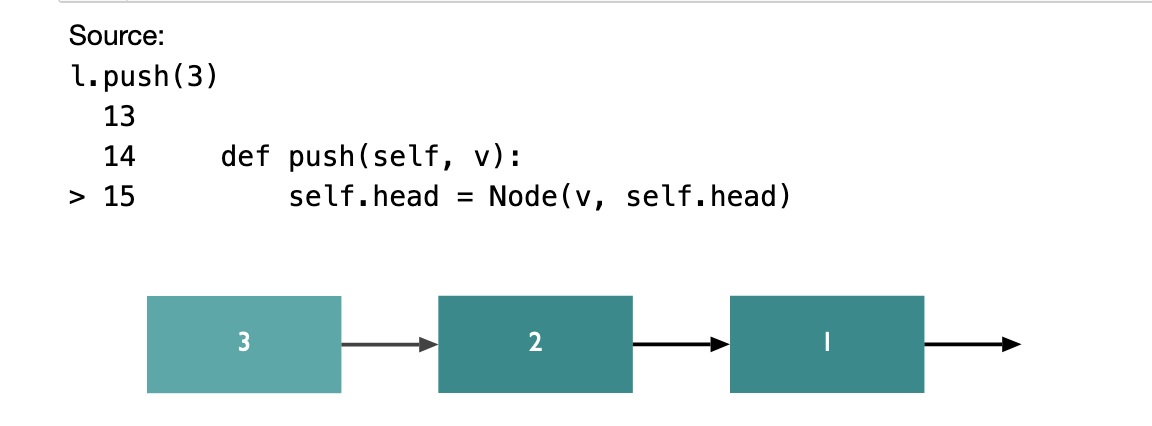
\includegraphics[width=\linewidth]{imagenes/ejemplos/ejemplo}
    \caption{Captura de la visualización generada a partir del código~\ref{lst:ejemplo-uso}.}
    \label{fig:visualizacion_ej}
    \centering
\end{figure}

Para registrar las operaciones primitivas sobre la estructura de datos el decorador \textit{node} modifica los campos pasados como parámetros para que al momento de acceder o asignar a estos campos se registre la operación en el \textit{logger}.

El \textit{logger} es un objeto que mantiene el registro de las operaciones primitivas sobre la estructura de datos. Además, se puede utilizar como un \textit{context manager} (objetos de Python que definen un contexto y se utilizan con \texttt{with}) y dentro del scope introducido todas las operaciones serán registradas en este logger. En el código~\ref{lst:ejemplo-logger-ctx-mgr} se puede ver un ejemplo de esta funcionalidad.

\begin{listing}[htb]
\caption{Ejemplo de uso del \textit{logger} como un \textit{context manager}.}
\label{lst:ejemplo-logger-ctx-mgr}
\begin{minted}[linenos=true]{python}
from dsvisualizer import logger

with Logger() as logger:
    n = Node(5, Node(10, Node(20, None)))
logger.visualize()

with logger:
    n = Node(10, n)
logger.visualize()
\end{minted}
\end{listing}

Cuando se aplica el decorador \textit{container} a una clase, se crea un Logger asociado a cada instancia de esa clase y para todos los métodos de esa clase se utiliza ese logger como \textit{context manager} para que las operaciones sobre la estructura de datos queden registrada en el logger del contenedor.
